\documentclass[11pt]{article}

\usepackage[a4paper,margin=1in]{geometry}
\usepackage[T1]{fontenc}
\usepackage[utf8]{inputenc}
\usepackage{lmodern}
\usepackage{graphicx}
\usepackage{booktabs}
\usepackage{tabularx}
\usepackage{array}
\usepackage{enumitem}
\usepackage{xcolor}
\usepackage{hyperref}
\usepackage{amsmath}

\definecolor{NSRAGNavy}{HTML}{0B1F33}
\definecolor{NSRAGTeal}{HTML}{1F7A8C}
\definecolor{NSRAGGold}{HTML}{F2A541}
\definecolor{NSRAGRed}{HTML}{C44536}
\definecolor{NSRAGGreen}{HTML}{2A9D8F}
\definecolor{NSRAGGray}{HTML}{4E5D6C}

\hypersetup{
    colorlinks=true,
    linkcolor=NSRAGTeal,
    urlcolor=NSRAGTeal,
    citecolor=NSRAGTeal
}

\title{\textbf{Neuro-Symbolic-RAG: A Multi-Hop Agent Framework for Verifiable Scientific Reasoning}\\
\large Codebase Review and Current Progress Report}
\author{Student Name \\ Project Submission Draft}
\date{April 7, 2026}

\begin{document}
\maketitle

\begin{abstract}
This paper documents the current state of the \textit{Neuro-Symbolic-RAG} (NSRAG) repository, a modular research prototype for multi-hop reasoning with explicit decomposition, hybrid retrieval, agentic hop execution, and formal verification. The codebase is organized as a phased pipeline: Phase 1 establishes a naive retrieval-augmented generation baseline, Phase 2 builds a symbolic query decomposer, Phase 3 adds a multi-head retrieval router, Phase 4 executes a multi-hop reasoning agent, and Phase 5 implements a verifier for hallucination control. The strongest achieved results are in the decomposition and retrieval layers, where the system reaches 100\% DAG validity on a 50-sample decomposition benchmark and 84.0 Recall@5 / 0.8027 MRR on a 200-sample retrieval benchmark. The end-to-end Phase 4 agent is implemented and evaluated, but it currently remains slightly below its acceptance target, reporting 8.8 exact match and 19.53 F1 on 500 HotpotQA samples. The codebase is therefore best described as a strong systems research prototype with a completed modular stack and a remaining controller-quality gap before it can claim a fully verified, production-grade multi-domain reasoning result.
\end{abstract}

\section{Introduction}
Multi-hop question answering and scientific reasoning systems fail for two recurring reasons: they retrieve relevant evidence but do not chain it correctly, or they generate plausible answers without enough grounding and verification. The NSRAG project addresses this by combining neural retrieval, symbolic structure, and verifiability in a single pipeline.

The motivating idea is strong: represent difficult questions as a graph of smaller sub-questions, route each hop through the most useful retrieval head, synthesize a short answer, and then verify the final output before returning it. This design is especially compelling for physics, mathematics, and research-heavy domains where exactness matters more than stylistic fluency.

This document is intentionally honest about the current state of the repository. It is not written as a claim of final SOTA performance. Instead, it is a submission-ready description of what the codebase already achieves, what remains incomplete, and why the project is still promising.

\section{What the Codebase Is}
The repository is organized into clear phase-based modules:

\begin{itemize}[leftmargin=1.2em]
\item \texttt{phase1/}: data download, FAISS indexing, and a naive RAG baseline over HotpotQA.
\item \texttt{phase2/}: a Groq-backed symbolic decomposer that converts a question into a typed DAG of sub-questions.
\item \texttt{phase3/}: a retrieval router with dense Qdrant retrieval, optional Neo4j graph retrieval, and SymPy-based symbolic solving.
\item \texttt{phase4/}: the NSRAG agent that executes hops in topological order and synthesizes a final answer.
\item \texttt{phase5/}: a formal verifier that applies equation checks, chain-of-verification prompts, and attribution tests.
\item \texttt{eval/}: shared exact match and F1 evaluation utilities.
\item \texttt{datasets/}, \texttt{benchmarks/}, \texttt{baselines/}, and \texttt{vector\_db/}: supporting corpora, benchmark loaders, and external tooling.
\end{itemize}

The codebase uses Groq-hosted LLM calls for decomposition and answer generation, BAAI \texttt{bge-base-en-v1.5} embeddings for dense retrieval, Qdrant for vector storage, optional Neo4j traversal for graph retrieval, and SymPy for symbolic computation and verification.

\subsection*{Why the design is neuro-symbolic}
The project is appropriately named \textit{neuro-symbolic} because it mixes:

\begin{itemize}[leftmargin=1.2em]
\item neural components: dense embeddings, LLM-based decomposition, LLM-based answer synthesis;
\item symbolic components: explicit DAG planning, dependency-aware hop execution, SymPy solving, and formal verification gates;
\item retrieval grounding: passage selection, evidence traces, and attribution-aware hallucination control.
\end{itemize}

\section{System Pipeline}
Figure~\ref{fig:architecture} shows the current architecture implemented in the repository.

\begin{figure}[h]
    \centering
    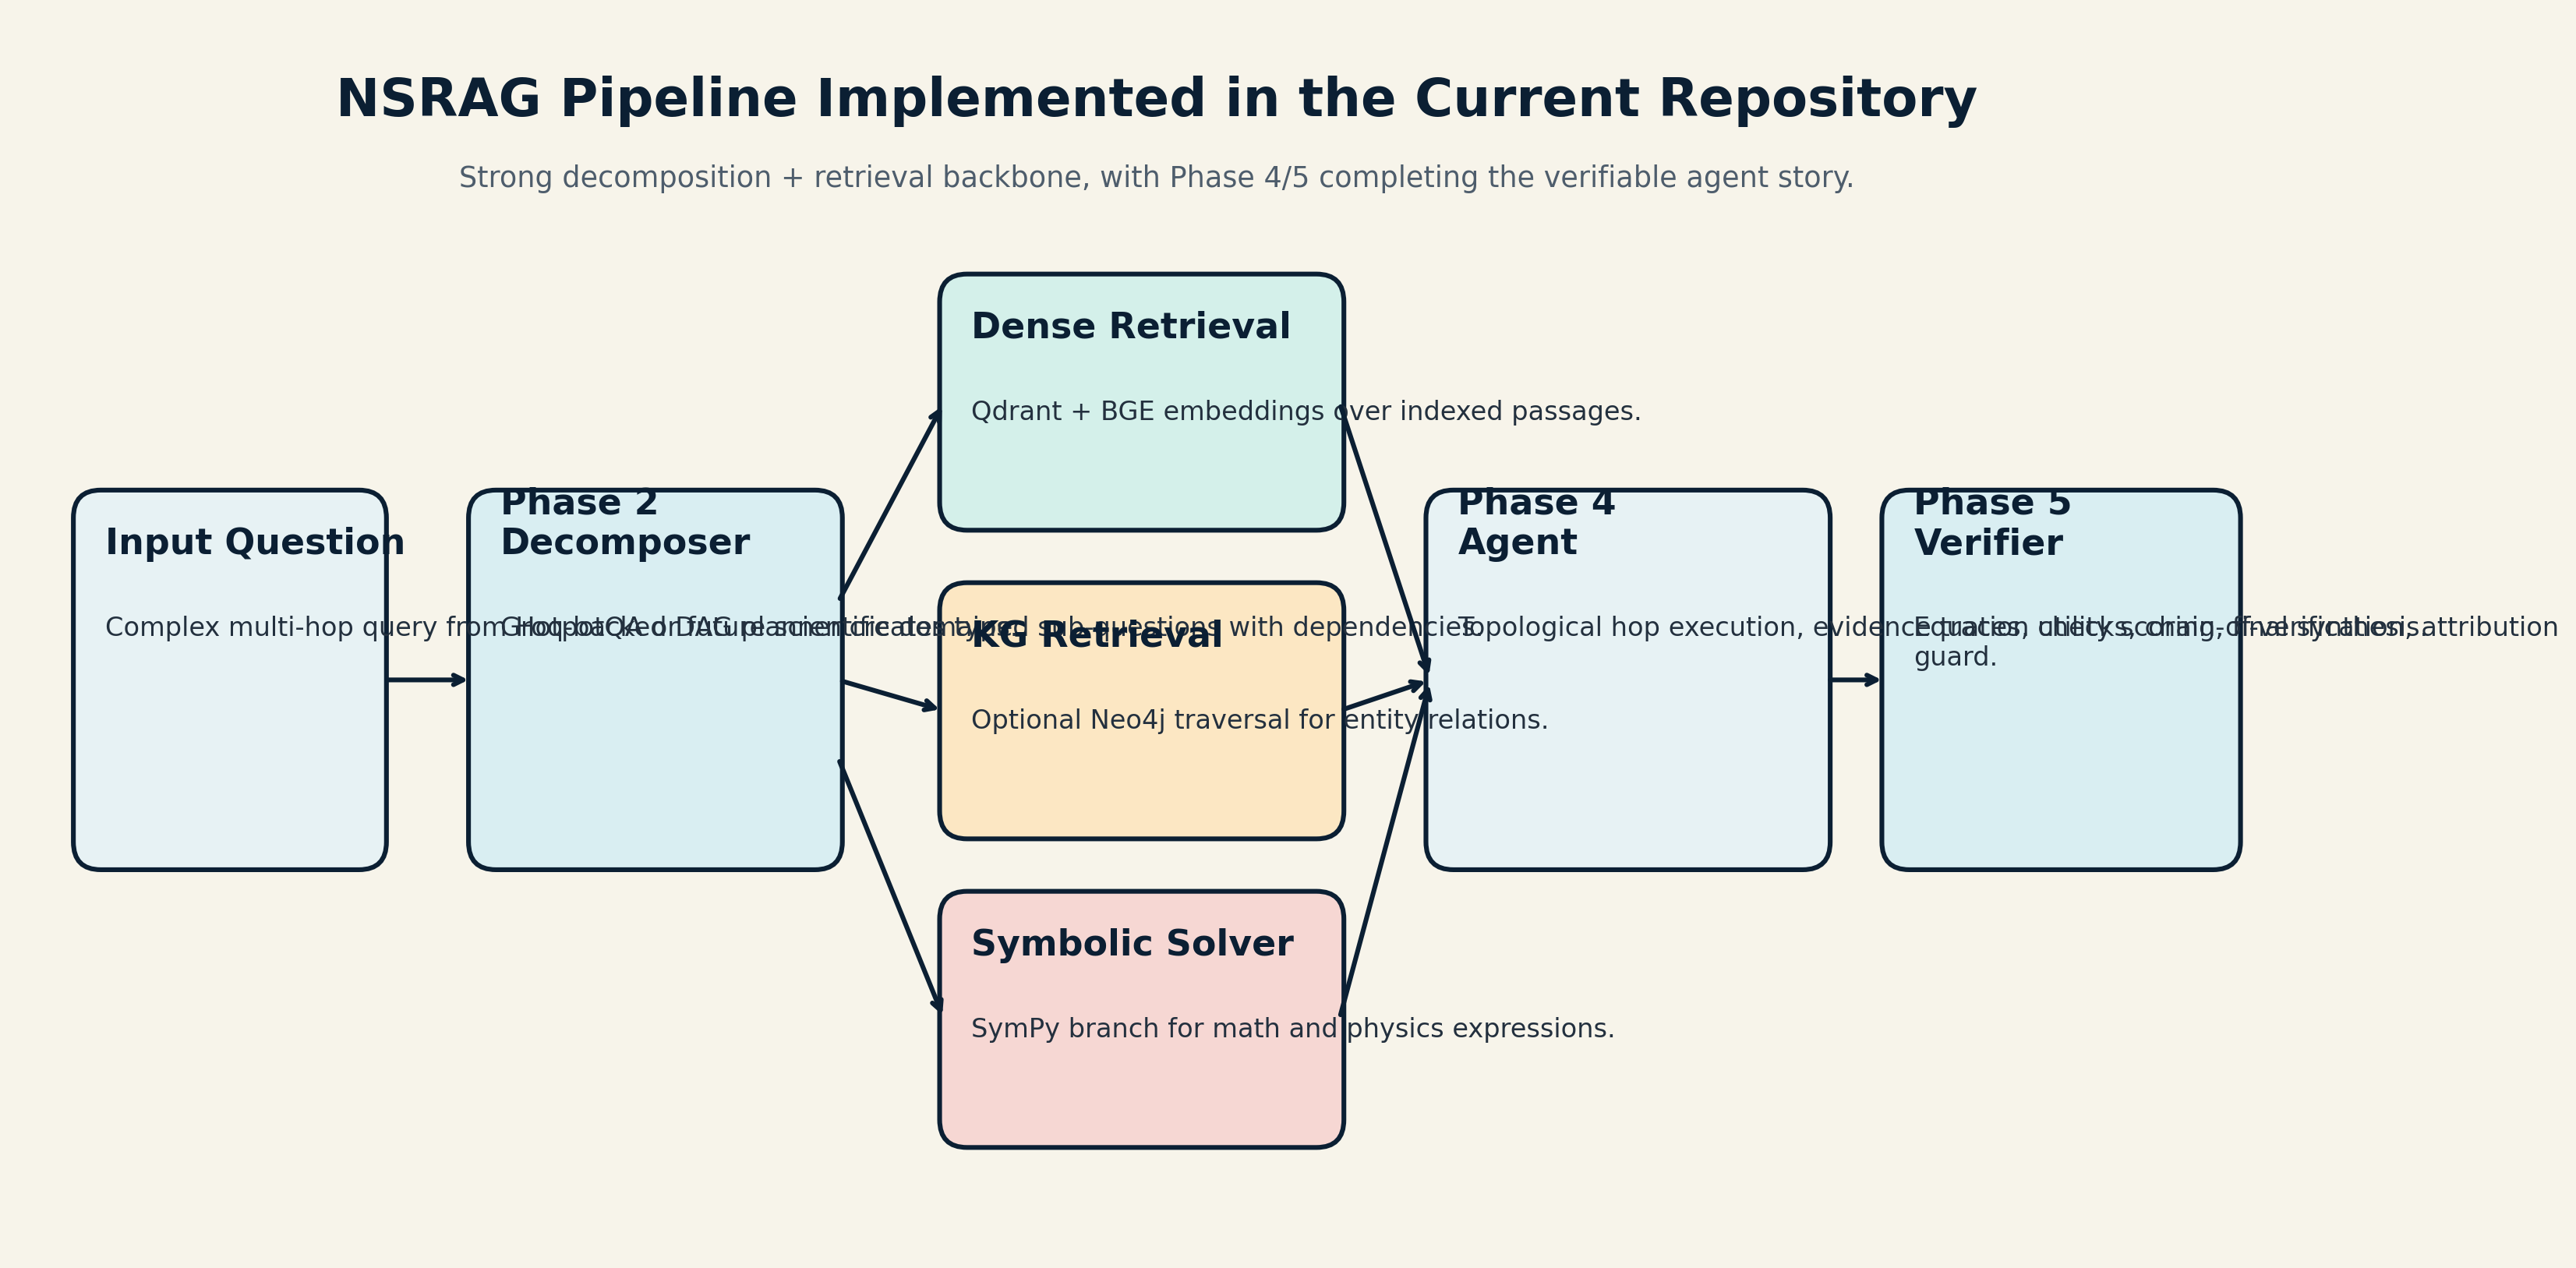
\includegraphics[width=\linewidth]{assets/nsrag_architecture.png}
    \caption{Current NSRAG pipeline implemented across phases 2--5.}
    \label{fig:architecture}
\end{figure}

The high-level flow is:

\begin{enumerate}[leftmargin=1.4em]
\item A complex question is decomposed into a small DAG of sub-questions.
\item Each sub-question is routed to retrieval heads based on domain and trigger rules.
\item Hop answers are produced in dependency order and accumulated into a reasoning trace.
\item A final short answer is synthesized from the hop trace.
\item A verifier checks equations, factual consistency, and attribution grounding.
\end{enumerate}

The architecture is conceptually strong, but the current code also reveals useful nuance:

\begin{itemize}[leftmargin=1.2em]
\item The early knowledge alignment routine exists in Phase 4 but is currently disabled to reduce API calls.
\item The retrieval layer stores sparse features and exposes optional graph and solver heads, but the default benchmark path is still dominated by dense retrieval.
\item Neo4j retrieval is graceful but optional; if Neo4j is not running, the graph head disables itself.
\item Phase 5 verification is implemented, but its full metrics are not yet present in the current workspace state.
\end{itemize}

\section{Phase-Wise Methodology}
\subsection{Phase 1: Naive RAG Baseline}
Phase 1 builds a local FAISS index over HotpotQA contexts and answers questions with a single retrieval-and-generate loop. This baseline is important because it provides a grounded reference point for the later agentic system. The baseline is intentionally simple: one dense retrieval pass, short context windows, and a concise answer-only generation prompt.

\subsection{Phase 2: Symbolic Query Decomposer}
Phase 2 converts the original question into a minimal DAG, typically with exactly two sub-questions. Each node is domain-tagged as \texttt{physics}, \texttt{math}, \texttt{chemistry}, \texttt{biology}, or \texttt{general}. This module is one of the best-performing parts of the system. It gives the overall framework interpretability and makes multi-hop execution explicit.

\subsection{Phase 3: Hybrid Retrieval Router}
Phase 3 introduces three retrieval heads:

\begin{itemize}[leftmargin=1.2em]
\item dense Qdrant retrieval over embedded passages;
\item optional Neo4j graph traversal for scientific entity relations;
\item SymPy-triggered symbolic solving for math and physics style questions.
\end{itemize}

This phase is especially valuable for the scientific framing of the project because it moves beyond plain text retrieval and allows a symbolic branch when equation-like questions are detected.

\subsection{Phase 4: NSRAG Agent}
Phase 4 is the controller layer. It runs decomposition, executes each hop in topological order, records evidence and confidence for every step, computes utility heuristics, and synthesizes a final answer. This is the most research-significant layer because it integrates everything into a reasoning agent.

At the same time, it is also the current bottleneck. The reported EM/F1 numbers show that the controller still loses too much accuracy between retrieval and final answer synthesis.

\subsection{Phase 5: Formal Verifier}
Phase 5 contains a verification stack with three gates:

\begin{itemize}[leftmargin=1.2em]
\item SymPy equation consistency checks for math/physics outputs,
\item chain-of-verification yes/no checks,
\item attribution overlap checks over the hop trace.
\end{itemize}

This is a strong research idea and a valuable differentiator for the project. However, the present submission should describe it as \textit{implemented and ready for evaluation}, not as a fully benchmarked achievement, because final verifier metrics are not yet saved in the current workspace.

\section{Experimental Setup and Current Results}
All reported numbers in this document come from repository artifacts already present in the workspace:

\begin{itemize}[leftmargin=1.2em]
\item \texttt{phase1/results/naive\_rag\_hotpotqa\_scores.json}
\item \texttt{phase2/results/decomposer\_eval\_metrics.json}
\item \texttt{phase3/results/retrieval\_metrics.json}
\item \texttt{phase4/results/nsrag\_hotpotqa\_metrics.json}
\end{itemize}

The main reported evaluation dataset is HotpotQA. Additional dataset preparation exists for MuSiQue, 2WikiMultiHopQA, and TheoremQA, but those broader cross-domain results are not yet fully reported in the current repo state.

\subsection{Phase summary}
\begin{table}[h]
\centering
\small
\begin{tabularx}{\linewidth}{>{\raggedright\arraybackslash}p{1.2cm} >{\raggedright\arraybackslash}p{3cm} >{\raggedright\arraybackslash}X >{\raggedright\arraybackslash}p{2.1cm}}
\toprule
\textbf{Phase} & \textbf{Module} & \textbf{Achieved Result} & \textbf{Status} \\
\midrule
1 & Naive RAG baseline & HotpotQA (1000 samples): EM 16.6, F1 35.32 & Complete \\
2 & Symbolic decomposer & 50 samples: DAG validity 100.0, hop accuracy within 1 = 100.0, domain accuracy 100.0 & Complete \\
3 & Hybrid retrieval & 200 samples: Recall@5 84.0, Recall@10 84.0, MRR 0.8027 & Complete \\
4 & NSRAG agent & 500 samples: EM 8.8, F1 19.53, average hops 2.02 & In progress \\
5 & Formal verifier & Code implemented; final evaluation metrics not yet saved in repo state & Pending evaluation \\
\bottomrule
\end{tabularx}
\caption{Project status at submission time.}
\end{table}

\subsection{Target versus achieved}
\begin{figure}[h]
    \centering
    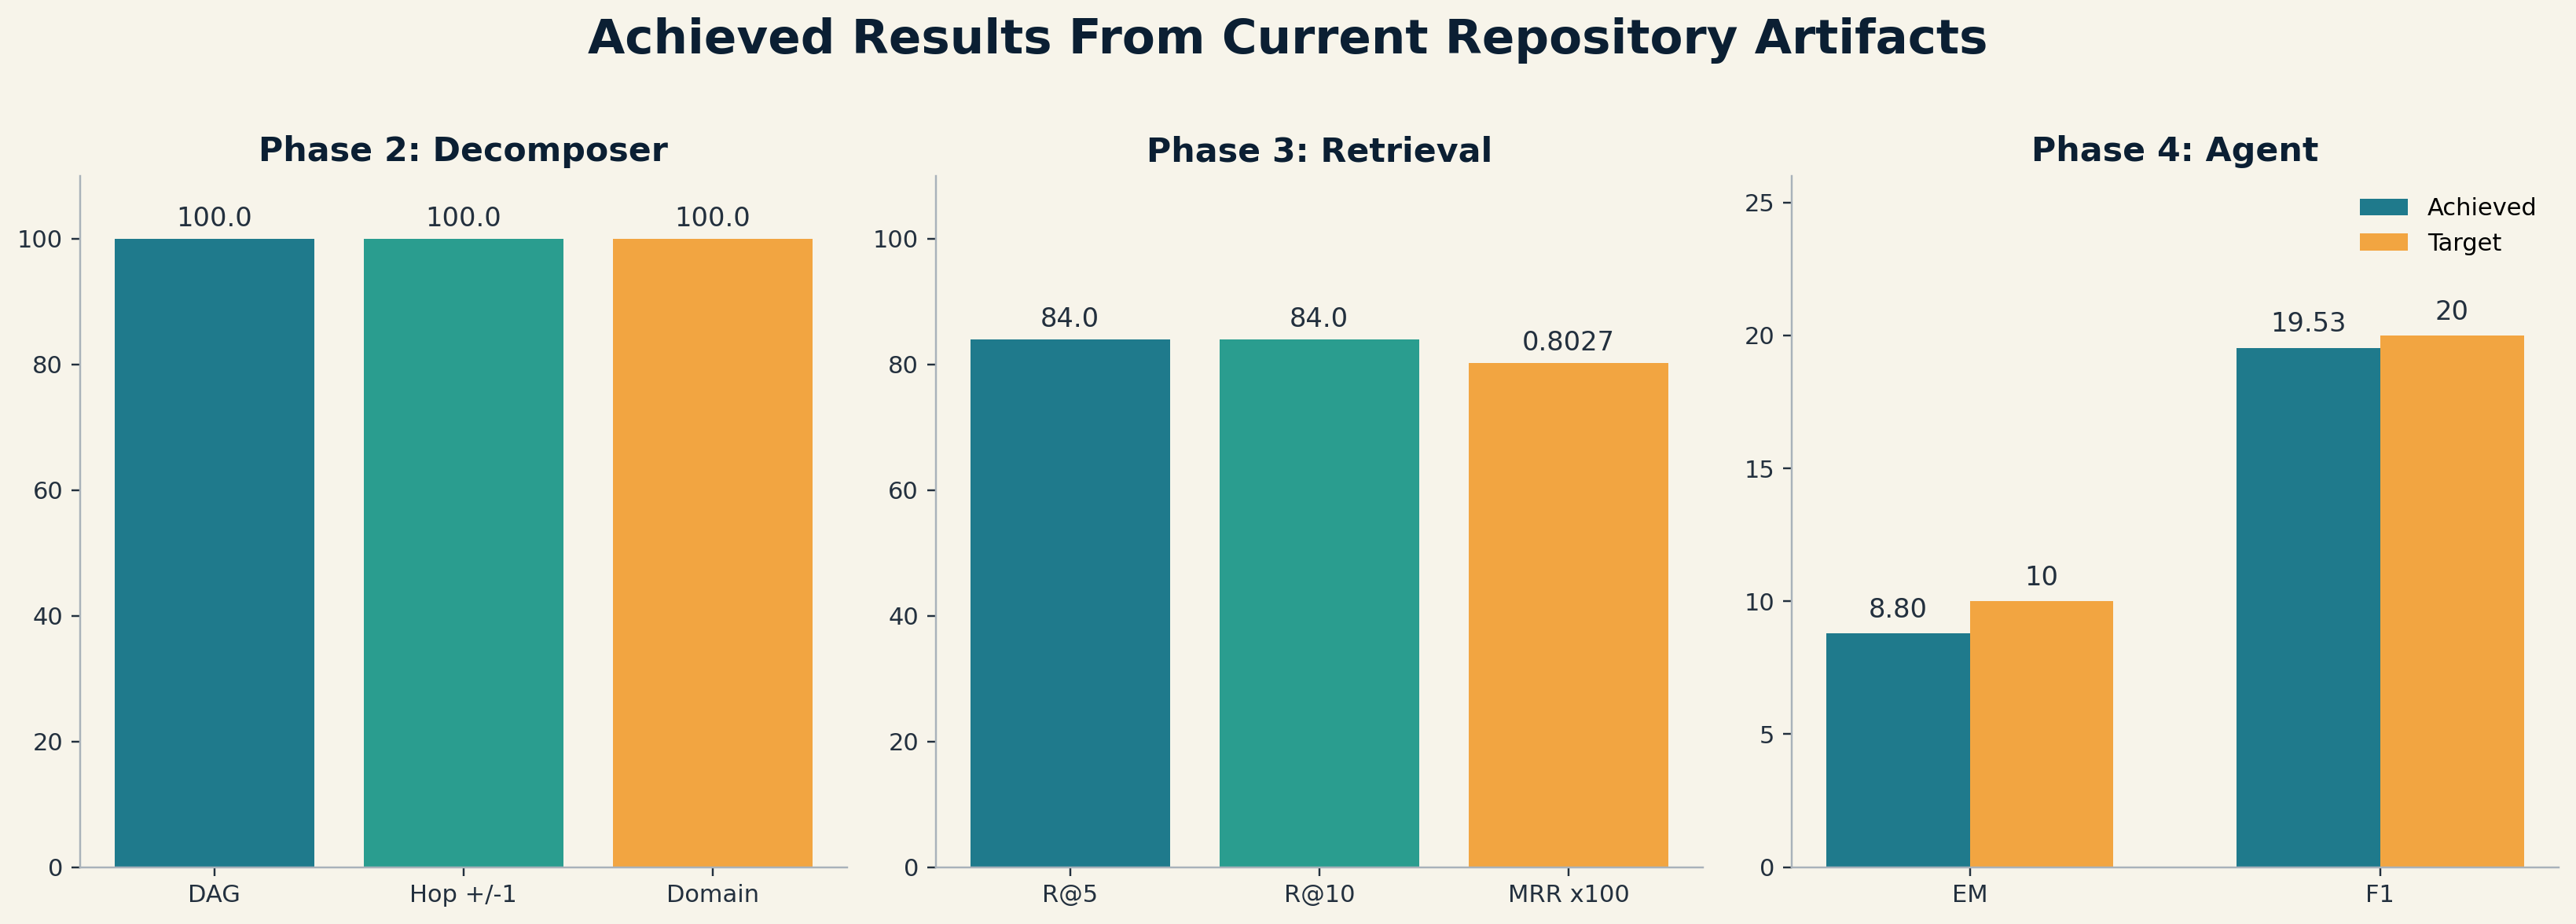
\includegraphics[width=\linewidth]{assets/nsrag_results_overview.png}
    \caption{Current achieved results across the strongest completed phases and the current Phase 4 gap.}
\end{figure}

The most important interpretation is straightforward:

\begin{itemize}[leftmargin=1.2em]
\item Phase 2 is strong and reliable.
\item Phase 3 is strong and comfortably usable.
\item Phase 4 is very close to its intended threshold, but not yet strong enough to claim end-to-end success.
\item The Phase 1 baseline still outperforms the current agent on HotpotQA answer quality.
\end{itemize}

This last point matters. The repository proves that the infrastructure exists, but it does not yet prove that the full agentic stack beats the simpler baseline on the main benchmark.

\section{Discussion: What Is Working and What Is Not}
\subsection{What is already working well}
Three parts of the project are already submission-worthy:

\begin{itemize}[leftmargin=1.2em]
\item \textbf{Modularity.} The phased architecture is easy to explain, extend, and debug.
\item \textbf{Interpretability.} The system stores sub-questions, dependencies, evidence titles, hop traces, and verification hooks.
\item \textbf{Research direction.} The combination of decomposition, retrieval routing, symbolic solving, and verification is a meaningful and timely research idea.
\end{itemize}

\subsection{Where the current bottleneck is}
The main weakness is the controller and final synthesis layer, not the project idea itself. Based on the code and saved results, the likely issues are:

\begin{itemize}[leftmargin=1.2em]
\item intermediate hops frequently return \texttt{UNKNOWN} even when retrieval finds partially useful evidence;
\item answer synthesis often produces near-correct but non-exact strings, which hurts exact match;
\item some retrieval heads are scaffolded but not yet fully fused into the main benchmark path;
\item the verification phase exists, but the project has not yet converted it into a completed empirical story.
\end{itemize}

In short, the system has strong backbone modules but still needs tighter orchestration to turn those modules into end-to-end gains.

\section{My Assessment of the Project}
This is a good project. In fact, it is better than many student repositories because it already has:

\begin{itemize}[leftmargin=1.2em]
\item a clean phase structure,
\item explicit acceptance gates,
\item reproducible metrics files,
\item multi-component reasoning traces,
\item a scientific-domain extension path,
\item and a verifier design rather than only a generator.
\end{itemize}

My honest view is that the project should be framed as a \textbf{serious prototype and progress-stage research system}, not as a fully finished multi-domain verified reasoner. That framing is still strong. The best story for submission is:

\begin{quote}
NSRAG already demonstrates reliable question decomposition, strong retrieval, modular neuro-symbolic routing, and a working end-to-end agent stack, while the final controller and verifier evaluation remain the final steps before a fully validated research result.
\end{quote}

That is an honest and compelling claim, and it matches the codebase.

\section{Recommended Submission Framing}
For a presentation or paper submission, the strongest wording is:

\begin{itemize}[leftmargin=1.2em]
\item emphasize the \textbf{architecture contribution} and the \textbf{phase-wise engineering validation};
\item report \textbf{achieved results as of now}, especially the decomposition and retrieval milestones;
\item describe Phase 4 as \textbf{implemented and near target}, not finished;
\item describe Phase 5 as \textbf{implemented verifier pipeline awaiting full benchmark reporting};
\item present multi-domain scientific reasoning as the \textbf{design objective already supported by the code}, while clearly stating that HotpotQA is the main benchmark with complete current metrics.
\end{itemize}

This lets the submission sound ambitious without overstating the evidence.

\section{Conclusion}
The NSRAG codebase is a well-structured neuro-symbolic multi-hop reasoning framework with clear research intent and real implementation depth. The repository already validates its decomposition and retrieval layers strongly, and it contains a complete path from question decomposition to formal verification. The current gap is that the Phase 4 agent has not yet converted that strong infrastructure into better end-to-end answer quality than the naive baseline. Therefore, the correct conclusion is not that the project is unfinished, but that it is \textbf{functionally built, empirically partial, and very close to becoming a convincing full-stack reasoning system}.

\vspace{0.7em}
\noindent\textbf{Practical note.} Before external sharing, ensure that any API keys in environment files are removed or rotated.

\end{document}
